\chapter{Hubble: an Industrial System for Audience Expansion in Mobile Marketing}

\textbf{Reference:}~\url{https://dl.acm.org/doi/pdf/10.1145/3394486.3403295}

\textbf{Keywords:} embeddings, lookalike, audience expansion, graphs, knowledge distillation

\section*{Какую задачу решают авторы?}

Авторы решают довольно популярную в области интернет-рекламы задачу --- расширение аудитории. \\

Часто, у рекламодателя может быть список пользователей, которые положительно отреагировали на предыдущую рекламную кампанию (seed множество).

Для того чтобы показывать новое объявление пользователям, которые с большей вероятностью совершат целевое действие, рекламная система может помочь рекламодателю и найти пользователей, которые похожи на seed множество. \\

На практике при решении данной задачи разработчики сталкиваются со следующим основным челенджем:

\begin{itemize}
    \item система должна хорошо масштабироваться на случай большого числа кампаний и пользователей, и выдавать расширенную аудиторию в течении нескольких минут
\end{itemize}

В рамках работы авторы описывают two-stage подход, где в оффлайне обучают эмбеддинги для пользователей и рекламных кампаний, и в онлайне обучают легковесные модели для расширения аудитории. 

Основным недостатков предыдущих работ~\cite{dewet2019finding,liu2019real} с two-stage подходом является недостаточно хорошее качество пользовательских эмбеддингов, которые не отражают все многообразие интересов пользователя. \\

В работе представлен ряд оффлайн и онлайн экспериментов, где показано превосходство нового метода над существующими state-of-the-art подходами к решению задачи расширения аудитории.

\section*{Как решают?}

Общая архитектура системы Hubble представлена на Рисунке~\ref{fig:hubble}

\begin{figure}[ht]
    \centering
    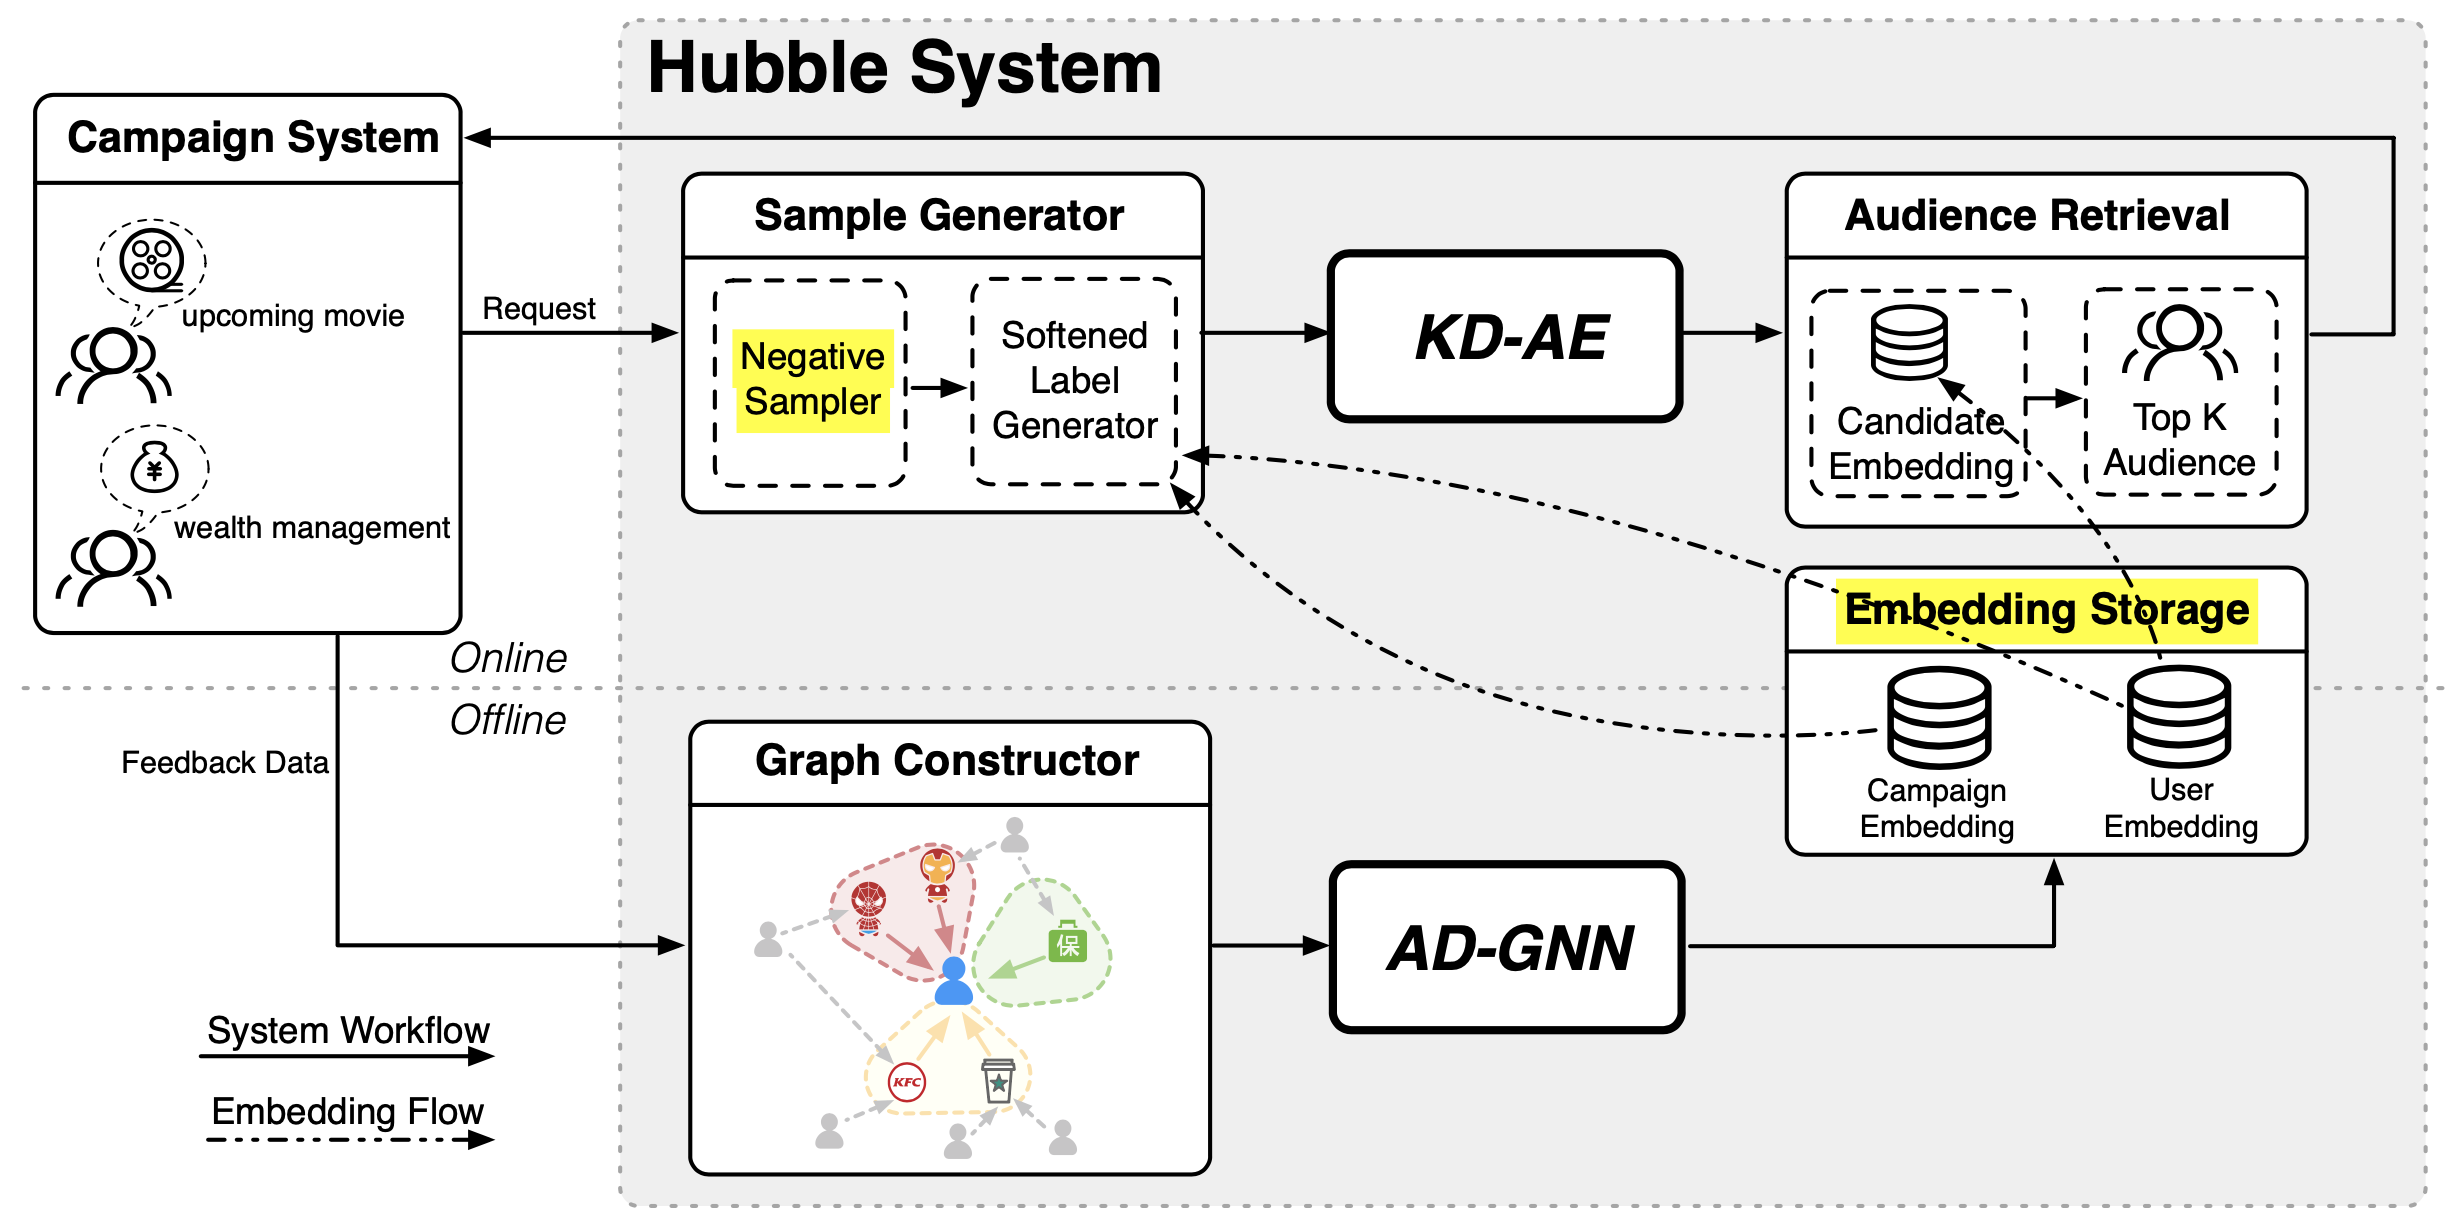
\includegraphics[width=0.8\linewidth]{images/hubble.png}
    \caption{\footnotesize{The architecture of Hubble System.}}
    \label{fig:hubble}
\end{figure}

Рассмотрим подробнее, что происходит в рамках онлайн и оффлайн фаз.

\subsection*{Offline Representation Learning}

В оффлайн части решения можно выделить две основные части: User-Campaign граф и модель AD-GNN для обучения эмбеддингов пользователей и кампаний.

\paragraph{User-Campaign граф} Данный граф по сути представляет из себя двудольный граф, в котором между пользователем и кампанией есть ребро, если пользователь совершил какое-то целивое действие, например, кликнул по объявлению, в рамках рекламной кампании. \\

Можно сказать, что данный граф содержит в себе информацию о различных комерческих интересах пользователя.

Если обучить эмбеддинги для вершин User-Campaign граф, то ожидается, что близкие эмбеддинги пользователей будут соответствовать пользователям с похожими интересами.

\paragraph{AD-GNN} Не вдаваясь в подробности архитектуры, рассмотрим как обучаются эмбеддинги для пользователей и рекламных кампаний. \\

Эмбеддинги обучаются на задаче \textit{link-prediction} --- пытаемся для пользователя $u$ и кампании $c$ обучить такие вектора $\vech_u, \vech_c$, что $y_{G} \coloneqq \sigma(\vech_u \vech_c)$ дает нам вероятность того, что между пользователем и кампанией есть ребро в графе. 

По сути $y_{G}$ принимает большое значение для близких векторов, и маленькое для далеких. \\

В качестве положительных примеров для обучения используются пары $(u, c)$ соотвествующие ребрам в User-Campaign графе, а в качестве негативных такие пары $(u', c')$, где пользователь $u'$ видел рекламу в рамках кампании $c'$, но не совершил целивое действие. \\

По сути перед нами задача бинарной классификации, поэтому во время обучения минимизируется обычный Binary Cross-Entropy Loss. \\

После того как были обучены эмбеддинги для пользователей и кампаний они загружаются в Embedding Storage (см. Рисунок~\ref{fig:hubble}).

\subsection*{Online Audience Expansion with Knowledge Distillation}

Система получает аудиторию $\mathcal{S}_c$, которую нужно расширить. Если для кампании $c$ уже есть эмбеддинг, то есть если она присуствует в User-Campaign графе, то для расширения аудитории достаточно найти пользователей с большим скором $\sigma(\vech_u \vech_c)$. \\

На практике, часто создаются новые кампании, для которых еще нет вершины в графе. В данной ситуации обучается классификатор, который предсказывает вероятность того, что пользователь совершит целевое действие.

Для обучения модели в онлайне генерируется множество случайных пользователей $\mathcal{U}_n \subset \mathcal{U} \setminus \mathcal{S}_c$ (см. Рисунок~\ref{fig:hubble}), и модель обучается на эмбеддингах различать пользователей из $\mathcal{S}_c$ от $\mathcal{U}_n$. \\

Для того чтобы в онлайн модель передать больше знаний от оффлайн модели AD-GNN, авторы используют \textit{knowledge distillation}, то есть обучают онлайн модель не только на \textit{hard} лэйблах (1 - если пользователь из $\mathcal{S}_c$ и 0 - в противном случае), но и на \textit{soft} лэйблах, которые получают от AD-GNN.

Soft лэйблы получают следующим образом.
\begin{enumerate}
    \item Выполняется поиск похожих кампаний на кампанию $c$. 
    Делается это с помощью разбиения пользователей из $\mathcal{S}_c$ на $k$ кластеров и последующим поиском наиболее похожей кампании на каждый кластер. В итоге получаем множество $\{c_i\}^{k}_{i=1}$ из $k$ кампаний.
    \item Soft label для пользователя - средняя похожесть на вектора для кампаний из множества  $\{c_i\}^{k}_{i=1}$.
\end{enumerate}

Итоговый лосс выглядит следующим образом:

\begin{align*}
    \mathcal{L}=&-\frac{1}{\left|\mathcal{D}\right|} \sum_{\left(u, y_{h}, y_{s}\right) \in \mathcal{D}} y_{h} \log \left(\hat{y}\right)+\left(1-y_{h}\right) \log \left(1-\hat{y}\right) \\
    &-\frac{\gamma}{\left|\mathcal{D}\right|} \sum_{\left(u, y_{h}, y_{s}\right) \in \mathcal{D}} y_{s} \log \left(\hat{y}\right)+\left(1-y_{s}\right) \log \left(1-\hat{y}\right) \\
    &+\frac{\lambda}{2}\left\|\Theta\right\|_{2} ,
\end{align*}
где $\hat{y} = MLP(\vech_u)$, $y_h$ - hard label, $y_s$ - soft label и $\gamma$ - гиперпараметр, который контролирует степень переноса знаний из AD-GNN в онлайн модель. \\

В рамках экспериментов авторы показывают, что при $\gamma > 0$ улучшается качество онлайн модели, то есть модель действительно получает дополнительное полезное знание от AD-GNN.

\subsection*{Experiments}

Во-первых, авторы показывают, что система работает лучше текущих state-of-the-art решений для задачи расширения аудитории.

Во-вторых, демонстрируют, что предложенная архитектура сети AD-GNN работает лучше других sota решений на задаче \textit{link-prediction}.

И наконец, показывают многократное ускорение по времени в онлайне, которое достигается в основном за счет того, что на вход моделе поступают эмбеддинги пользователей, размерность которых существенно меньше размерности обычного описания с помощью фичей --- 64 vs 300k.

\section*{Мое мнение}

Тут \url{https://vk.com/@papersreaders-finding-users-who-act-alike-transfer-learning-for-expanding} можно почитать конспект статьи от Pinterest с KDD'19, в которой описано решение~\cite{dewet2019finding}.